% IA 642 Defensive Security
% Week 03 Module 01 Lab: Segment and Instrument Meridian's Network
% Submit as: Ali_Usama_Week03_Module01_Lab.pdf
\documentclass[11pt,letterpaper]{article}

\usepackage[margin=0.75in]{geometry}
\usepackage{array}
\usepackage{booktabs}
\usepackage{tabularx}
\usepackage{xltabular}
\usepackage{needspace}
\usepackage{enumitem}
\usepackage{parskip}
\usepackage{ragged2e}
\usepackage{titlesec}
\usepackage{hanging}
\usepackage{graphicx}
\usepackage{float}
\usepackage{placeins}
\usepackage{microtype}
\usepackage{xcolor}
\usepackage{colortbl}
\usepackage{listings}
\usepackage{caption}
\usepackage[colorlinks=true,linkcolor=blue,citecolor=blue,urlcolor=blue]{hyperref}
\usepackage{xurl}

\hypersetup{pdfauthor={Unais Ali; Hafiz Usama}, pdftitle={IA 642 Week 03 Lab 3.1 Meridian Network}}

\definecolor{tblhead}{HTML}{1F4E79}
\definecolor{tblrow}{HTML}{F0F4F8}
\definecolor{codebg}{HTML}{F7FAFC}
\setlength{\parindent}{0pt}
\renewcommand{\arraystretch}{1.22}
\setlength{\tabcolsep}{3.5pt}
\newcommand{\labtablesetup}{%
  \footnotesize
  \setlength{\tabcolsep}{4pt}%
  \renewcommand{\arraystretch}{1.28}%
}
\raggedbottom
\setlist[itemize]{leftmargin=1.2em,itemsep=0.25em,topsep=0.35em,parsep=0pt}
\setlist[enumerate]{leftmargin=1.3em,itemsep=0.35em,topsep=0.35em,parsep=0pt}
\newcolumntype{Y}{>{\RaggedRight\arraybackslash}X}
\newcolumntype{L}[1]{>{\RaggedRight\arraybackslash}p{#1}}
\titleformat{name=\section,numberless}{\large\bfseries\color{tblhead}}{}{0em}{}
\titlespacing*{name=\section,numberless}{0pt}{0.85em}{0.3em}
\titleformat{name=\subsection,numberless}{\normalsize\bfseries\color{tblhead}}{}{0em}{}
\titlespacing*{name=\subsection,numberless}{0pt}{0.55em}{0.2em}

% Keep Part/Step headings with following content (no orphan headings)
\newcommand{\labpart}[1]{%
  \par\vspace{0.15em}%
  \Needspace{10\baselineskip}%
  \section*{#1}%
  \nopagebreak
}
\newcommand{\labstep}[1]{%
  \Needspace{8\baselineskip}%
  \subsection*{#1}%
  \nopagebreak
}
\newcommand{\labpartbig}[1]{%
  \par\vspace{0.15em}%
  \Needspace{22\baselineskip}%
  \section*{#1}%
  \nopagebreak
}

\newcommand{\aparef}[2]{\hyperref[ref:#1]{#2}}
\newcommand{\refitem}[1]{\phantomsection\label{ref:#1}}

\lstset{
  basicstyle=\ttfamily\footnotesize,
  backgroundcolor=\color{codebg},
  frame=single,
  rulecolor=\color{tblhead},
  breaklines=true,
  columns=fullflexible,
  keepspaces=true,
  showstringspaces=false,
  xleftmargin=0.4em,
  xrightmargin=0.4em,
  aboveskip=0.5em,
  belowskip=0.5em
}

\begin{document}

\begin{center}
{\large\textbf{EASTERN MICHIGAN UNIVERSITY}}\\[0.12em]
{\normalsize College of Engineering and Technology}\\[0.25em]
{\Large\textbf{IA 642: Defensive Security}}\\[0.15em]
{\large\textbf{Week 03, Module 01 Lab: Segment and Instrument Meridian's Network}}\\[0.2em]
{\small Network Defense Architecture \& Detection \quad\textbullet\quad Lab 3.1}
\end{center}

\vspace{0.35em}\hrule\vspace{0.45em}

\begin{tabularx}{\textwidth}{@{}L{3.2cm}Y L{2.0cm}Y@{}}
\textbf{Group members} & Unais Ali & \textbf{EID} & E02805019 \\
 & Hafiz Usama &  & E02574092 \\
\textbf{Course} & IA 642 Defensive Security & \textbf{Week} & 3, Lab 3.1 \\
\textbf{Case} & Meridian Health Network & \textbf{Date} & September 2026 \\
\end{tabularx}

\vspace{0.35em}
\textit{This lab continues the Meridian Health Network case. It microsegments the EHR/PHI Core, chooses telemetry at each zone boundary, writes signature and behavioral detections, and states honest coverage gaps for encrypted command-and-control.}

{\footnotesize
\noindent\textbf{Terms used.}
Electronic Health Record (EHR);
Protected Health Information (PHI);
Transmission Control Protocol (TCP);
Hypertext Transfer Protocol Secure (HTTPS);
Transport Layer Security (TLS);
mutual Transport Layer Security (mTLS);
Test Access Point (TAP);
Switched Port Analyzer (SPAN);
Intrusion Detection System (IDS);
Intrusion Prevention System (IPS);
Packet Capture (PCAP);
IP Flow Information Export (IPFIX);
Network Detection and Response (NDR);
Payment Card Industry (PCI);
Cardholder Data Environment (CDE);
Server Message Block (SMB);
Domain Name System (DNS);
Server Name Indication (SNI);
Endpoint Detection and Response (EDR);
National Institute of Standards and Technology (NIST);
Internet Engineering Task Force (IETF);
Request for Comments (RFC).
}

\vspace{0.25em}
\labpart{Part A: Extend the Segmentation}

\labstep{Step 1: Microsegment the EHR / PHI Core}

Segmentation controls traffic between zones, whereas microsegmentation applies workload-level rules between systems inside the same zone. This design follows Zero Trust principles by avoiding implicit trust based only on network location and granting only the least-privilege access required between specific workloads \aparef{nist}{(NIST, 2020)}. If one workload is compromised, these restrictions reduce the attacker's ability to move laterally to other systems.

\textbf{Design assumption.} Because the scenario does not specify Meridian's exact EHR technology stack, the workload names and application protocols below represent a realistic example architecture; PostgreSQL is assumed for the patient-record database.

\begingroup\labtablesetup
\begin{xltabular}{\textwidth}{@{}L{2.15cm}L{2.25cm}L{2.05cm}L{1.9cm}Y@{}}
\toprule
\rowcolor{tblhead}
\textcolor{white}{\textbf{Source}} &
\textcolor{white}{\textbf{Destination}} &
\textcolor{white}{\textbf{Port / Protocol}} &
\textcolor{white}{\textbf{Enforcement}} &
\textcolor{white}{\textbf{Allowed Because}} \\
\endfirsthead
\toprule
\rowcolor{tblhead}
\textcolor{white}{\textbf{Source}} &
\textcolor{white}{\textbf{Destination}} &
\textcolor{white}{\textbf{Port / Protocol}} &
\textcolor{white}{\textbf{Enforcement}} &
\textcolor{white}{\textbf{Allowed Because}} \\
\endhead
\midrule
EHR web front-end &
EHR application layer &
TCP 443 / HTTPS &
Service-mesh sidecar with mTLS &
The web front-end must send authenticated EHR application requests to the application/API service. mTLS allows the services to authenticate each other while encrypting the service-to-service connection. \\
EHR Application/API Server &
Patient Records Database &
TCP 5432 / PostgreSQL &
Hypervisor filter &
The EHR application needs database access to retrieve and update patient records. Only the EHR application workload is permitted to initiate database connections. \\
EHR Application/API Server &
Audit / Logging Server &
TCP 6514 / Syslog over TLS &
Host-based firewall &
The EHR application must send security and audit events to the centralized logging server. The logging server's host firewall permits this logging traffic from the authorized EHR application workload only. \\
EHR web front-end &
Audit / Logging Server &
TCP 6514 / Syslog over TLS &
Host-based firewall &
The web front-end must send access, authentication, and security logs to the audit server for monitoring and investigation. \\
EHR backup server &
Patient Records Database &
TCP 5432 / PostgreSQL &
Hypervisor filter &
The authorized backup workload needs controlled access to the patient database so protected health information can be backed up. Other workloads are not permitted to use this database path. \\
\bottomrule
\end{xltabular}
\endgroup

\textbf{Default-deny policy.} All other workload-to-workload communication inside the EHR/PHI Core that is not explicitly listed above is denied by default. Each permitted path is limited to the specific source workload, destination workload, port, and protocol required for normal operation.

\labstep{Step 2: Name the East-West Path You Are Most Worried About}

The east-west path of greatest concern is within the EHR/PHI Core, from the EHR Application/API Server to the Patient Records Database. If the application server were compromised, an attacker could abuse its legitimate database access to retrieve, modify, or potentially delete sensitive patient records and PHI. Because both workloads are inside the same EHR/PHI zone, the zone firewall alone would not prevent this lateral activity. Microsegmentation at the workload level is therefore important for limiting the application server to only the specific database access required for normal EHR operations.

\labpart{Part B: Choose Your Telemetry}

\labstep{Step 3: Telemetry Selection per Boundary}

\begin{figure}[H]
\centering
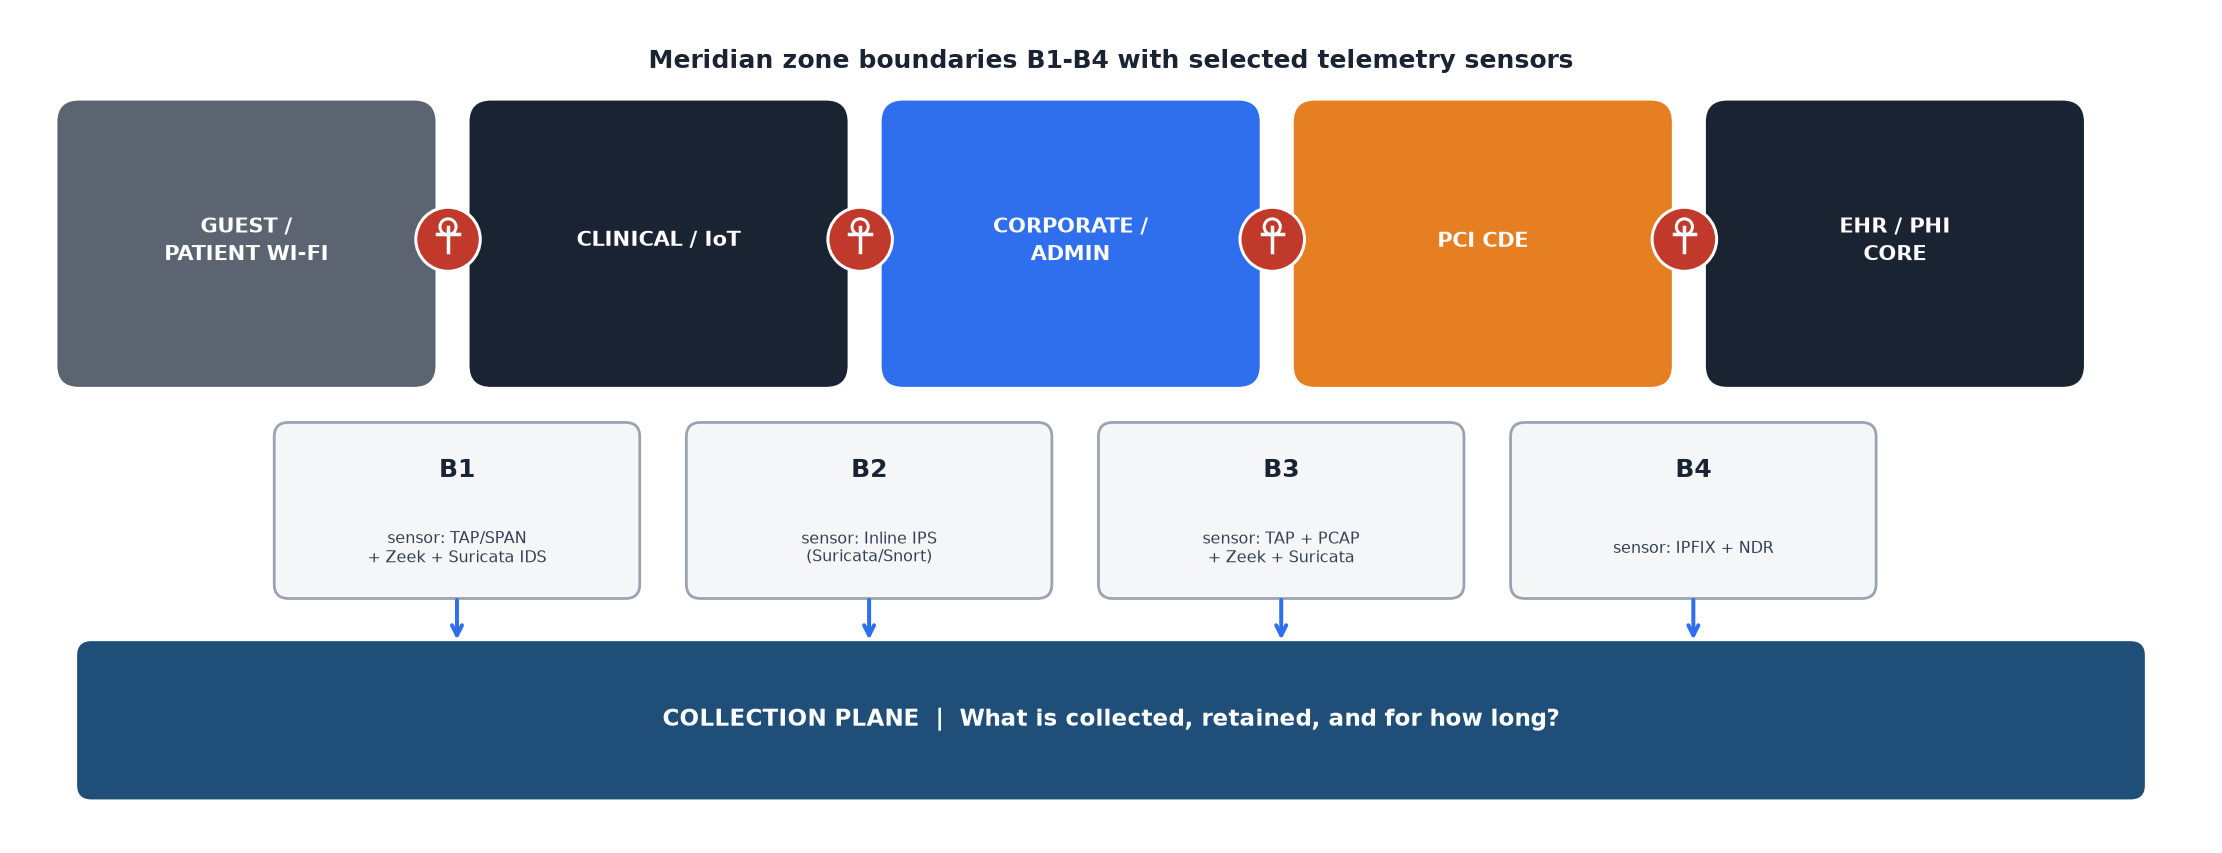
\includegraphics[width=\textwidth]{figures/fig_meridian_boundaries.png}
\caption{Meridian zone boundaries B1--B4 with selected telemetry sensors feeding the collection plane.}
\label{fig:boundaries}
\end{figure}

\begingroup\labtablesetup
\rowcolors{2}{white}{tblrow}
\begin{tabularx}{\textwidth}{@{}L{2.6cm}L{2.3cm}L{2.5cm}L{1.7cm}Y@{}}
\toprule
\rowcolor{tblhead}
\textcolor{white}{\textbf{Boundary}} &
\textcolor{white}{\textbf{Zone it separates}} &
\textcolor{white}{\textbf{Telemetry chosen}} &
\textcolor{white}{\textbf{Retention}} &
\textcolor{white}{\textbf{Why This, Here}} \\
\midrule
B1: TAP/SPAN + Zeek + passive Suricata IDS &
Guest/Patient Wi-Fi $\leftrightarrow$ Clinical/IoT &
TAP/SPAN feeding Zeek protocol logging and a passive Suricata IDS &
30 days of Zeek logs and IDS alerts &
Guest/patient Wi-Fi is untrusted and may generate large traffic volumes, so passive monitoring avoids putting an inline device in the path of clinical systems. Zeek provides connection, DNS, and TLS metadata, while Suricata can run the B1 signature rule from Step~5. \\
B2: Inline IPS &
Clinical/IoT $\leftrightarrow$ Corporate/Admin &
Inline Suricata/Snort-compatible IPS + alert/event logging &
90 days of alerts/logs &
Traffic between clinical devices and corporate systems should be tightly constrained. Unexpected cross-zone sessions represent high-risk lateral movement. The inline IPS can run the B2 signature rule, identify prohibited traffic, and stop it while retaining alerts rather than all packet payloads. \\
B3: TAP + selective PCAP + Zeek + passive Suricata IDS &
Corporate/Admin $\leftrightarrow$ PCI CDE &
TAP feeding selective full packet capture, Zeek protocol logs, and a passive Suricata IDS &
7 days PCAP; 90 days Zeek logs and IDS alerts &
The PCI boundary protects the cardholder data environment. Short-term PCAP provides forensic evidence, Zeek provides structured protocol metadata, and Suricata can run the B3 signature rule from Step~5. \\
B4: IPFIX + NDR &
PCI CDE $\leftrightarrow$ EHR/PHI Core &
IPFIX + NDR behavioral analytics &
90 days &
IPFIX, standardized in RFC~7011, provides a mechanism for exporting network flow information to a collector \aparef{ipfix}{(IETF RFC 7011)}. In this design, Meridian's exported flow records will include source and destination addresses, ports, timestamps, duration, packet counts, and byte counts while avoiding retention of packet payloads. NDR can analyze those records for unusual relationships, fixed-interval beaconing, and abnormal traffic patterns over time. \\
\bottomrule
\end{tabularx}
\endgroup

\textbf{Corporate Internet-egress instrumentation.} In addition to the four required internal zone boundaries B1--B4, Meridian's Corporate/Admin Internet egress will export IPFIX to the NDR platform and provide a TAP/SPAN feed to Zeek. IPFIX and the relevant Zeek connection, TLS, and DNS logs will be retained for at least 90 days, providing the 30-day history required for behavioral baselining while preserving additional investigation history. This telemetry is necessary to detect the Thursday BILL-WS-14 outbound TLS behavior described in Steps~7 and~9.

\labstep{Step 4: Justify One Thing You Deliberately Will Not Collect}

\begingroup\labtablesetup
\rowcolors{2}{white}{tblrow}
\begin{tabularx}{\textwidth}{@{}L{2.4cm}L{2.6cm}Y Y@{}}
\toprule
\rowcolor{tblhead}
\textcolor{white}{\textbf{Rejected Source}} &
\textcolor{white}{\textbf{Where It Would Have Gone}} &
\textcolor{white}{\textbf{What It Would Have Caught}} &
\textcolor{white}{\textbf{Why You Rejected It}} \\
\midrule
Continuous full packet capture (PCAP) &
B4: PCI CDE $\leftrightarrow$ EHR/PHI Core &
Complete packet-level evidence for traffic crossing the EHR boundary, including replayable session details and payload visibility when traffic is not encrypted. &
Continuous PCAP would create excessive storage cost and unnecessary privacy exposure by retaining traffic associated with highly sensitive patient information. IPFIX and behavioral analytics provide timing, volume, source/destination, and connection-pattern visibility without retaining PHI payloads. The blind spot is that analysts cannot fully reconstruct historical packet payloads at B4 when only flow records are retained. \\
\bottomrule
\end{tabularx}
\endgroup

\labpart{Part C: Write the Signature Detections}

\labstep{Step 5: Three Rules}

\textbf{Policy rationale.} The three rules below target traffic Meridian has defined as prohibited. Guest/Patient Wi-Fi should never initiate sessions into Clinical/IoT systems; Clinical/IoT devices should never initiate arbitrary sessions into Corporate/Admin systems; and direct SMB access from ordinary Corporate/Admin hosts into the PCI CDE is prohibited because administrative access to the CDE should occur only through approved management paths.

\begingroup\labtablesetup
\rowcolors{2}{white}{tblrow}
\begin{tabularx}{\textwidth}{@{}L{0.5cm}L{2.8cm}L{1.4cm}Y Y@{}}
\toprule
\rowcolor{tblhead}
\textcolor{white}{\textbf{\#}} &
\textcolor{white}{\textbf{Boundary}} &
\textcolor{white}{\textbf{Rule}} &
\textcolor{white}{\textbf{What It Fires On}} &
\textcolor{white}{\textbf{What It Would Miss}} \\
\midrule
1 &
B1: Guest/Patient Wi-Fi $\leftrightarrow$ Clinical/IoT &
Rule 1 &
An established TCP session initiated from Guest/Patient Wi-Fi toward any Clinical/IoT host. &
UDP/ICMP traffic, non-established attempts, attacks occurring entirely inside the Clinical zone, and malicious activity using other permitted paths. \\
2 &
B2: Clinical/IoT $\leftrightarrow$ Corporate/Admin &
Rule 2 &
An established TCP session initiated from a Clinical/IoT host toward a Corporate/Admin host. &
UDP/ICMP traffic, Corporate-initiated traffic in the opposite direction, intra-zone attacks, and malicious traffic using other allowed paths. \\
3 &
B3: Corporate/Admin $\leftrightarrow$ PCI CDE &
Rule 3 &
An established SMB session from Corporate/Admin to the PCI CDE on TCP 445. &
Attacks using other protocols or ports, malicious HTTPS, and attacks occurring entirely inside the CDE. \\
\bottomrule
\end{tabularx}
\endgroup

\begin{lstlisting}[caption={Suricata/Snort signature rules for B1, B2, and B3},label={lst:rules}]
# Rule 1 -- B1 Guest/Patient Wi-Fi -> Clinical/IoT
alert tcp $GUEST_NET any -> $CLINICAL_NET any (
    msg:"B1 POLICY VIOLATION - Guest host initiated TCP session to Clinical/IoT";
    flow:to_server,established;
    classtype:policy-violation;
    threshold:type limit, track by_src, count 1, seconds 300;
    sid:1000101;
    rev:1;
)

# Rule 2 -- B2 Clinical/IoT -> Corporate/Admin
alert tcp $CLINICAL_NET any -> $CORP_NET any (
    msg:"B2 POLICY VIOLATION - Clinical/IoT host initiated TCP session to Corporate/Admin";
    flow:to_server,established;
    classtype:policy-violation;
    threshold:type limit, track by_src, count 1, seconds 300;
    sid:1000102;
    rev:1;
)

# Rule 3 -- B3 Corporate/Admin -> PCI CDE SMB
alert tcp $CORP_NET any -> $PCI_NET 445 (
    msg:"B3 POLICY VIOLATION - Corporate host initiated SMB session to PCI CDE";
    flow:to_server,established;
    classtype:policy-violation;
    threshold:type limit, track by_src, count 1, seconds 300;
    sid:1000103;
    rev:1;
)
\end{lstlisting}

\labstep{Step 6: Test Your Rules Against the Incident}

No, none of the three signature rules would have fired on the 143 Thursday-night sessions. The rules monitor specific prohibited internal behaviors at B1, B2, and B3, while the incident involved a Corporate/Admin billing workstation initiating permitted TLS connections to an external Internet host on TCP 443. The traffic therefore did not match the source, destination, and protocol conditions defined by these rules, and the encrypted session also provided no known payload signature for the IDS to match. This demonstrates why behavioral detection is needed to identify the repeated timing, near-identical session size, and unusual new external relationship that signatures alone would miss.

\labpart{Part D: Design the Behavioral Detections}

\labstep{Step 7: Two Behavioral Detections}

\noindent\textbf{Detection 1: Periodic low-volume outbound beaconing}

\begingroup\labtablesetup
\begin{tabularx}{\textwidth}{@{}L{3.6cm}Y@{}}
\toprule
\rowcolor{tblhead}
\textcolor{white}{\textbf{Field}} &
\textcolor{white}{\textbf{Detail}} \\
\midrule
Detection logic &
Alert when a Corporate/Admin workstation makes at least 6 outbound TLS sessions to the same external destination within 60 minutes, at approximately 8-minute $\pm$ 2-minute intervals, with each session under 5~KB, and the destination has not appeared in that host's prior 30-day history. This detection is designed to catch the Thursday incident. \\
\rowcolor{tblrow}
Telemetry required &
Corporate/Admin Internet-egress IPFIX + NDR, enriched with the Zeek TAP/SPAN feed selected in Part~B. \\
Baseline needed &
30 days of normal external destinations, connection frequency, timing, byte counts, ports, and normal working hours. \\
\rowcolor{tblrow}
Expected false positives &
Software-update agents, monitoring/management agents, cloud-sync tools, or other legitimate applications that periodically check in to a vendor service. \\
\bottomrule
\end{tabularx}
\endgroup

\vspace{0.6em}
\noindent\textbf{Detection 2: Abnormal B4 EHR/PHI relationship}

\begingroup\labtablesetup
\begin{tabularx}{\textwidth}{@{}L{3.6cm}Y@{}}
\toprule
\rowcolor{tblhead}
\textcolor{white}{\textbf{Field}} &
\textcolor{white}{\textbf{Detail}} \\
\midrule
Detection logic &
Alert when a source crossing B4 establishes 5 or more sessions within 15 minutes to an EHR/PHI destination not seen in its previous 30-day baseline, or transfers more than $3\times$ its normal hourly byte volume to that EHR/PHI destination. \\
\rowcolor{tblrow}
Telemetry required &
B4 IPFIX + NDR behavioral analytics. \\
Baseline needed &
30 days of normal source/destination relationships, connection frequency, ports, timing, and byte volume across B4. \\
\rowcolor{tblrow}
Expected false positives &
New approved integrations, scheduled synchronization, maintenance activity, disaster-recovery testing, or newly provisioned services. \\
\bottomrule
\end{tabularx}
\endgroup

\labstep{Step 8: The Baseline Problem}

The primary risk is baseline poisoning: malicious activity may already exist within Meridian's 30-day learning period and could therefore be incorporated into the model of normal behavior. A compromised host's abnormal destinations, connection timing, or traffic volume could then appear normal and reduce the sensitivity of future NDR detections. Meridian should validate the baseline period against IDS/IPS alerts, incident records, EDR findings, and threat-intelligence data and exclude known or suspected compromise periods before training the model. The baseline should also be continuously reviewed and updated rather than treated as permanently trustworthy.

\labpartbig{Part E: Detect Without Decrypting}

\labstep{Step 9: One Encrypted-Traffic Detection}

\begingroup\labtablesetup
\begin{xltabular}{\textwidth}{@{}L{4.0cm}Y@{}}
\toprule
\rowcolor{tblhead}
\textcolor{white}{\textbf{Element}} &
\textcolor{white}{\textbf{Answer}} \\
\endfirsthead
\toprule
\rowcolor{tblhead}
\textcolor{white}{\textbf{Element}} &
\textcolor{white}{\textbf{Answer}} \\
\endhead
\midrule
1. Observable signal you are keying on &
Repeated low-volume outbound TLS sessions from the same Corporate/Admin workstation to the same external destination, occurring at a nearly fixed interval and representing a destination relationship not previously seen for that host. Use source/destination IP, TCP 443, timestamps, byte and packet counts, duration, direction, and TLS metadata. \\
2. Telemetry or log that carries it &
Corporate/Admin Internet-egress IPFIX $\rightarrow$ NDR plus TAP/SPAN $\rightarrow$ Zeek, as selected in Part~B. IPFIX supplies flow timing, volume, source/destination, ports, packets, and duration; Zeek provides connection and TLS metadata, including SNI/certificate context where observable and JA3/JA3S fingerprints. \\
3. Threshold/comparison that turns it into a detection &
Alert when a Corporate/Admin workstation establishes 6 or more TLS sessions to the same external destination within 60 minutes, approximately 8 minutes $\pm$ 2 minutes apart, each under 5~KB, and the destination has not appeared in its previous 30-day baseline. This would detect the Thursday pattern of 143 near-identical sessions. \\
4. Role JA3/JA3S fingerprinting plays &
JA3/JA3S is supporting evidence, not the sole trigger. A fingerprint unique or rare within Meridian increases confidence when combined with the fixed timing and new relationship, but it does not by itself prove malicious activity \aparef{ja3}{(Althouse, Atkinson, \& Atkins, 2017)}. \\
5. One benign activity that would also trigger it &
A legitimate endpoint-management or software-update agent could periodically contact the same vendor service using small TLS sessions and resemble beaconing. \\
6. What an analyst should do first when it fires &
Correlate the Corporate/Admin IPFIX/NDR records with Zeek connection, TLS, and DNS context for BILL-WS-14. Check the destination, SNI/domain, JA3/JA3S fingerprint, timing pattern, and 30-day history to determine whether the traffic belongs to an approved application before concluding that it is malicious. \\
\bottomrule
\end{xltabular}
\endgroup

\labstep{Step 10: The Limits of the Fingerprint}

A JA3 fingerprint seen on only one Meridian host is a strong investigative lead because it shows that the host's TLS client behavior is unusual within the environment, but it is not proof of malicious activity. One benign explanation is that BILL-WS-14 runs a legitimate specialized billing or vendor application that uses a TLS library not used by other Meridian systems. A second explanation is that the workstation is running a different or newly updated version of legitimate software or its TLS library, causing a different ClientHello fingerprint. The fingerprint should therefore be correlated with the IPFIX flow pattern, destination, Zeek TLS/DNS context, and other available evidence before concluding that the traffic is malicious.

\labpartbig{Part F: Coverage and Honest Gaps}

\labstep{Step 11: Detection Coverage Map}

\begingroup\labtablesetup
\begin{xltabular}{\textwidth}{@{}L{3.0cm}L{1.9cm}L{2.6cm}Y@{}}
\toprule
\rowcolor{tblhead}
\textcolor{white}{\textbf{Technique}} &
\textcolor{white}{\textbf{Covered?}} &
\textcolor{white}{\textbf{Which Detection}} &
\textcolor{white}{\textbf{Confidence and Why}} \\
\endfirsthead
\toprule
\rowcolor{tblhead}
\textcolor{white}{\textbf{Technique}} &
\textcolor{white}{\textbf{Covered?}} &
\textcolor{white}{\textbf{Which Detection}} &
\textcolor{white}{\textbf{Confidence and Why}} \\
\endhead
\midrule
T1071: Application Layer Protocol &
Partially detected &
Step~7 Detection~1 and Step~9 encrypted-traffic detection &
The design detects some suspicious HTTPS/application-layer activity when it shows unusual timing, low volume, a new destination relationship, or unusual TLS characteristics. It may miss application-layer C2 that closely matches normal timing, destinations, session sizes, and TLS behavior \aparef{attack}{(MITRE ATT\&CK)}. \\
T1572: Protocol Tunneling &
Not detected &
None of the current detections specifically identify tunneling &
No current rule or behavioral detection specifically identifies an inner protocol being carried inside an allowed outer protocol or looks for protocol-log mismatches. Therefore tunneling could pass through an allowed protocol without triggering the current design. \\
T1090: Proxy &
Partially detected &
Step~9 encrypted-traffic detection &
Step~9 may identify proxy-mediated command-and-control when a Corporate/Admin host establishes a new, repeated, low-volume TLS relationship with an external intermediary that matches the behavioral threshold. However, the telemetry generally reveals only the immediate proxy endpoint rather than the true destination behind it, and use of a legitimate or previously known proxy with normal-looking timing and traffic volume could evade the detection. \\
\bottomrule
\end{xltabular}
\endgroup

\labstep{Step 12: Name What You Still Cannot See}

One attack this design could still miss is command-and-control from a compromised Corporate/Admin workstation over HTTPS to a legitimate cloud service that Meridian already uses regularly. If the attacker uses irregular connection timing, normal-sized sessions, an already-known destination, and the workstation's normal browser or operating-system TLS stack, the activity may not satisfy the Step~7 periodic-beacon threshold or any of the Part~C signature rules, and its JA3/JA3S fingerprint may provide no unusual supporting evidence. From the network perspective, the sessions could therefore closely resemble legitimate encrypted business traffic even though malicious commands are being carried inside them. This gap could be reduced by deploying endpoint detection and response (EDR) on Corporate/Admin workstations and correlating outbound network connections with the process, executable, user, and parent-process activity that created them. That endpoint context would help analysts distinguish an approved application connection from a suspicious process using the same legitimate HTTPS destination.

\section*{References}
\begin{hangparas}{1.5em}{1}
\refitem{nist}National Institute of Standards and Technology. (2020). \textit{SP 800-207: Zero Trust Architecture}. \url{https://csrc.nist.gov/pubs/sp/800/207/final}

\refitem{ipfix}Internet Engineering Task Force. (2013). \textit{RFC 7011: Specification of the IP Flow Information Export (IPFIX) Protocol}. \url{https://www.rfc-editor.org/rfc/rfc7011}

\refitem{pci}PCI Security Standards Council. \textit{Guidance for PCI DSS Scoping and Segmentation}. \url{https://www.pcisecuritystandards.org}

\refitem{cis}Center for Internet Security. \textit{CIS Critical Security Controls v8}, Control 12: Network Infrastructure Management and Control 13: Network Monitoring and Defense. \url{https://www.cisecurity.org/controls/v8}

\refitem{ja3}Althouse, J., Atkinson, J., \& Atkins, J. (2017). \textit{JA3 and JA3S TLS Client/Server Fingerprinting}. \url{https://github.com/salesforce/ja3}

\refitem{attack}MITRE Corporation. \textit{MITRE ATT\&CK Techniques T1071, T1572, and T1090}. \url{https://attack.mitre.org}
\end{hangparas}

\end{document}
